\renewcommand{\picturefontsize}{\LARGE}
\renewcommand{\pictureLineWidth}{0.8mm}

% For every picture that defines or uses external nodes, you'll have to
% apply the 'remember picture' style. To avoid some typing, we'll apply
% the style to all pictures.
\tikzstyle{every picture}+=[remember picture]
\tikzstyle{na} = [baseline=-.5ex]

\def\localarrow{
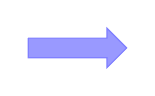
\begin{tikzpicture}
\path[draw=blue!50,fill=blue!40] (0,0.125) -- (1.0,0.125) -- (1.0,0.25) -- (1.25,0.0) -- (1.0,-0.25) -- (1.0,-0.125) -- (0.0,-0.125) -- (0.0,0.125);
\end{tikzpicture}
}

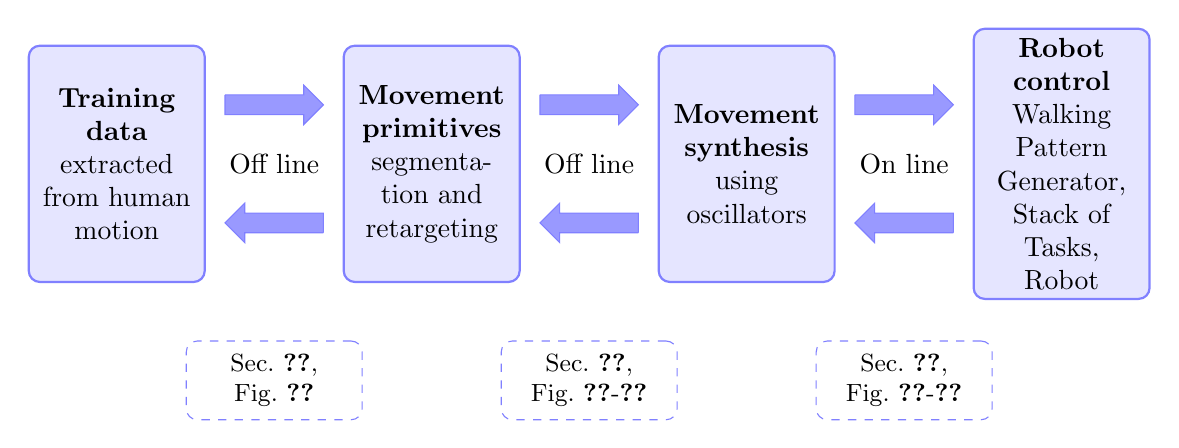
\begin{tikzpicture}%[show background grid]% every node/.style={draw,outer sep=0pt,thick}]

% Rectangle
\node (trainingdata) [text centered, shape=rectangle,rounded corners,draw=blue!50,fill=blue!10,thick,text width=2cm, minimum height=3cm]
  at (0.0,-0.5) {\textbf{Training data} extracted from human motion};

\node (movementprimitives) [text centered, shape=rectangle,rounded corners,draw=blue!50,fill=blue!10,thick,text width=2cm, minimum height=3cm]
  at (4.0,-0.5) {\textbf{Movement primitives} segmentation and retargeting};

\node (movementsynthesis) [text centered, shape=rectangle,rounded corners,draw=blue!50,fill=blue!10,thick,text width=2cm, minimum height=3cm]
  at (8.0,-0.5) {\textbf{Movement synthesis} using oscillators};

\node (robotcontrol) [text centered, shape=rectangle,rounded corners,draw=blue!50,fill=blue!10,thick,text width=2cm, minimum height=3cm]
  at (12.0,-0.5) {\textbf{Robot control}\\Walking Pattern Generator,\\ Stack of Tasks,\\ Robot};

\node (firstarrow) at (2.0,0.25) {\localarrow };

\node (trainingdatalabel) [text centered, shape=rectangle,rounded corners,draw=blue!50,fill=white,dashed,text width=2cm, minimum height=1cm,font=\small]
  at (2.0,-3.25)  {Sec.~\ref{subsec:modeling}, Fig.~\ref{fig:real}};

\node (sndarrow) at (6.0,0.25) {\localarrow };

\node (motionsynthesislabel) [text centered, shape=rectangle,rounded corners,draw=blue!50,fill=white,dashed,text width=2cm, minimum height=1cm,font=\small]
  at (6.0,-3.25) {Sec.~\ref{subsec:modeling}, Fig.~\ref{fig:Sources}-\ref{fig:RobotHuman}};

\node (thrdarrow) at (10.,0.25) {\localarrow };

\node (robotlabel)  [text centered, shape=rectangle,rounded corners,draw=blue!50,fill=white,dashed,text width=2cm, minimum height=1cm,font=\small]
  at (10.0,-3.25) {Sec.~\ref{sc:Implementation}, Fig.~\ref{fig:onlineWPG}-\ref{fig:zmpmb}};

\node[rotate=180] (rfirstarrow) at (2.0,-1.25) {\localarrow };
\node[rotate=180] (rsndarrow) at (6.0,-1.25) {\localarrow };
\node[rotate=180] (rthrdarrow) at (10.,-1.25) {\localarrow };

\node (offline1) at ( 2.0,-0.5) {Off line};
\node (offline2) at ( 6.0,-0.5) {Off line};
\node (offline1) at (10.0,-0.5) {On line};

\end{tikzpicture}
